\documentclass[tikz, border=5mm]{standalone}
\usetikzlibrary{arrows.meta, positioning}

\begin{document}
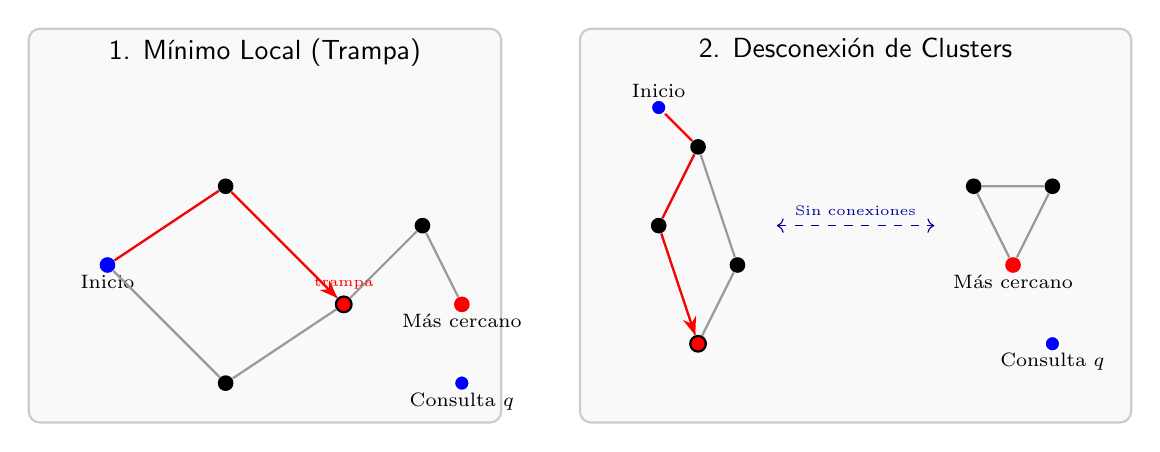
\begin{tikzpicture}[font=\sffamily, panel/.style={draw=black!20, fill=gray!5, rounded corners, thick}, node style/.style={circle, fill=black, inner sep=2pt}, query style/.style={circle, fill=blue, inner sep=2pt, draw=white, thick}, trap node/.style={circle, fill=red, inner sep=2pt, draw=black, thick}, edge style/.style={thick, black!40}, path edge/.style={->, >=Stealth, thick, red}]

    % =========================================================================
    % CUADRO 1: Mínimo Local Minimalista (6 nodos)
    % =========================================================================
    \draw[panel] (0, 0) rectangle (6, 5);
    \node[anchor=north] at (3, 5) {1. Mínimo Local (Trampa)};

    % Nodos
    \node[node style, blue] (n1) at (1, 2) {};
    \node[below, font=\scriptsize] at (n1) {Inicio};
    \node[node style] (n2) at (2.5, 3) {};
    \node[node style] (n3) at (2.5, 0.5) {};
    \node[trap node] (n4) at (4, 1.5) {}; % El mínimo local
    \node[node style] (n5) at (5, 2.5) {};
    \node[node style, red] (n6) at (5.5, 1.5) {};
    \node[below, font=\scriptsize] at (n6) {Más cercano};
    \node[query style] (q) at (5.5, 0.5) {};
    \node[below, font=\scriptsize] at (q) {Consulta $q$};

    % Aristas
    \draw[edge style] (n1) -- (n2) -- (n4) -- (n3) -- (n1);
    \draw[edge style] (n4) -- (n5) -- (n6);

    % Ruta Greedy que se detiene
    \draw[path edge] (n1) -- (n2) -- (n4);
    \node[above=2pt, font=\tiny, red] at (n4) {trampa};

    % =========================================================================
    % CUADRO 2: Partición de Clusters y Desconexión
    % =========================================================================
    \draw[panel] (7, 0) rectangle (14, 5);
    \node[anchor=north] at (10.5, 5) {2. Desconexión de Clusters};

    % Cluster A (Izquierda)
    \node[node style] (a1) at (8, 2.5) {}; \node[node style] (a2) at (8.5, 3.5) {};
    \node[node style] (a3) at (9, 2) {}; \node[trap node] (a4) at (8.5, 1) {};
    \draw[edge style] (a1)--(a2)--(a3)--(a4)--(a1);
    
    % Cluster B (Derecha - contiene respuesta)
    \node[node style] (b1) at (12, 3) {}; \node[node style] (b2) at (13, 3) {};
    \node[node style, red] (best3) at (12.5, 2) {};
    \node[below, font=\scriptsize] at (best3) {Más cercano};
    \node[query style] (consulta) at (13, 1) {};
    \node[below, font=\scriptsize] at (consulta) {Consulta $q$};
    \draw[edge style] (b1)--(b2)--(best3)--(b1);

    % Consulta q en Cluster A
    \node[query style] (Inicio) at (8, 4) {};
    \node[above, font=\scriptsize] at (Inicio) {Inicio};

    % Ruta que se queda atrapada en A
    \draw[path edge] (Inicio) -- (a2) -- (a1) -- (a4);
    
    % Indicación visual de la brecha
    \draw[<->, dashed, blue!60!black] (9.5, 2.5) -- (11.5, 2.5) node[midway, above, font=\tiny] {Sin conexiones};

\end{tikzpicture}
\end{document}